\documentclass[11pt]{article}
\usepackage[a4paper,margin=0.86in]{geometry}
\usepackage{amsmath,amssymb,amsthm,mathtools}
\usepackage{booktabs,array}
\usepackage{graphicx}
\usepackage{xcolor}
\usepackage{xurl}
\usepackage[hidelinks]{hyperref}
\hypersetup{
  pdftitle={Orthogonal Spectral Fan-Out Costs k(L-1) States},
  pdfauthor={Lluis Eriksson},
  pdfsubject={Exact global memory laws for passive rational-inner spectral routing}
}
\usepackage[nameinlink,capitalise]{cleveref}
\usepackage{microtype}
\usepackage{etoolbox}
\AtBeginEnvironment{thebibliography}{\footnotesize\setlength{\itemsep}{0pt}\setlength{\parsep}{0pt}}

\newtheorem{theorem}{Theorem}[section]
\newtheorem{proposition}[theorem]{Proposition}
\newtheorem{lemma}[theorem]{Lemma}
\newtheorem{corollary}[theorem]{Corollary}
\theoremstyle{definition}
\newtheorem{definition}[theorem]{Definition}
\newtheorem{example}[theorem]{Example}
\theoremstyle{remark}
\newtheorem{remark}[theorem]{Remark}
\newtheorem{limitation}[theorem]{Limitation}

\newcommand{\C}{\mathbb C}
\newcommand{\D}{\mathbb D}
\newcommand{\T}{\mathbb T}
\newcommand{\tr}{\operatorname{tr}}
\newcommand{\rank}{\operatorname{rank}}
\newcommand{\ran}{\operatorname{ran}}
\newcommand{\diag}{\operatorname{diag}}
\newcommand{\Span}{\operatorname{span}}
\newcommand{\dd}{\mathrm d}
\newcommand{\e}{\mathrm e}
\newcommand{\mcdeg}{\deg_{\mathrm{McM}}}
\newcommand{\nminus}{\nu_{-}}
\newcommand{\norm}[1]{\lVert#1\rVert}

\title{Orthogonal Spectral Fan-Out Costs $k(L-1)$ States:\\
A Global Memory Law Beyond Pairwise Routing}
\author{Lluis Eriksson}
\date{10 August 2026}

\begin{document}
\maketitle

\begin{abstract}
A passive lossless network may route the same $k$-dimensional input channel to
different output subspaces at different frequencies.  Every two-frequency
restriction can be cheap while the joint task is not.  We prove an exact
global law.  Let $L\ge2$, let $\zeta_1,\ldots,\zeta_L$ be distinct boundary frequencies
and let the $L$ prescribed output $k$-planes be mutually orthogonal.  Among
square finite rational-inner transfer matrices regular at the nodes, the
minimum McMillan degree is
\[
                         d_{\min}=k(L-1).
\]
Each pair alone has degree $k$, so the largest two-node minimum underestimates
the global memory by the unbounded factor $L-1$.  The result is independent of
node spacing.  Necessity has two proofs: a zero budget for one analytic
minor, and a Pick--Stein displacement identity whose negative inertia cannot
exceed realization rank.  Sufficiency follows from an explicit positive
completion
\[
 P_0=\bigl(C-\lambda_{\min}(C)I_L\bigr)\otimes I_k,
 \qquad
 C_{ij}=\frac{1}{1-\overline\zeta_i\zeta_j}\quad(i\ne j),
\]
followed by a lurking-isometry colligation.  For regular-polygon nodes the
completion spectrum is exactly $\{0,1,\ldots,L-1\}$, each repeated $k$
times.

The displacement proof yields a more general certificate: for calibrated
target-frame Gram matrix $G$, every interpolant satisfies
$\mcdeg S\ge\nminus(\mathbf1\mathbf1^*\otimes I_k-G)$.  Consequently the
full $k(L-1)$ bound survives whenever $\norm{G-I}<1$, and noisy estimates give
a fail-closed eigenvalue count.  Summing endpoint-only Grassmann speed limits
certifies only $\lceil kL/2\rceil$ states; the exact global law is
asymptotically twice as large.  Deterministic code tests arbitrary nodes, synthesizes minimal
multichannel colligations, and is replayed by an independent verifier.
\end{abstract}

\noindent\textbf{Keywords:} rational inner matrix; McMillan degree;
boundary Nevanlinna--Pick interpolation; Stein identity; matrix inertia;
Wigner--Smith delay; spectral routing; passive network.

\section{A global task hidden from every pair}

Consider one fixed input subspace observed at several frequencies.  At each
frequency a lossless transfer sends it to a prescribed output subspace.  The
two-node problem is governed by canonical angles, proper-delay action and a
finite rational degree \cite{ErikssonDelayRegions2026,
ErikssonActionMemory2026}.  It is tempting to replace a multi-node task by
its largest two-node restriction.  This paper gives an exact family for
which that surrogate loses an arbitrarily large factor.

The phenomenon is not geometric distance alone.  Mutually orthogonal output
planes are pairwise maximally separated, but each pair is realizable with
only $k$ states.  The global obstruction comes from requiring all pairwise
kernel blocks to belong to one positive Gram matrix.  Its size is measured
by the negative inertia of a Stein displacement before the unknown diagonal
blocks are chosen.

Boundary matrix interpolation, minimal rational interpolation, Pick matrices,
lurking isometries and their rank--degree correspondence are classical
\cite{AntoulasEtAl1990,BallKang1990,BolotnikovDym2006,BallKim1994,BallBolotnikov2018,
GombaniMichaletzky2007}.  Subspace all-pass interpolation and nodewise
group-delay design are also established \cite{BharathEtAl2023}.  We compared
the theorem statements and construction objectives of the closest sources.
Bolotnikov--Dym supply the boundary Schur and Stein framework; Ball--Kim and
Gombani--Michaletzky analyze stability and degree for general rational
interpolation; Bharath et al. construct boundary subspace all-pass filters by
choosing positive group-delay blocks.  None of these comparisons yielded the
orthogonal free-diagonal rank formula, the exact pairwise/global ratio, or the
operator-norm robust inertia certificate.  Our priority claim is restricted
to those explicit specializations.  The rank--degree proposition below is a
finite-dimensional corollary of classical realization theory, not a new
general Pick theorem.

\begin{table}[t]
\centering
\small
\begin{tabular}{@{}>{\raggedright\arraybackslash}p{0.24\linewidth}
>{\raggedright\arraybackslash}p{0.31\linewidth}
>{\raggedright\arraybackslash}p{0.35\linewidth}@{}}
\toprule
Source & Established ingredient & Added here \\
\midrule
Bolotnikov--Dym \cite{BolotnikovDym2006}
& Boundary matrix Schur interpolation, Stein identity and realizations
& Exact $k(L-1)$ orthogonal fan-out rank and robust inertia reading \\
Ball--Kim; Gombani--Michaletzky \cite{BallKim1994,GombaniMichaletzky2007}
& McMillan-degree questions for rational interpolants
& Node-independent closed formula for this subspace family \\
Bharath et al.\ \cite{BharathEtAl2023}
& Subspace all-pass synthesis and delay optimization
& Unbounded separation between the largest pair task and the joint task \\
Preceding resource laws \cite{ErikssonRouting2026,ErikssonDelayRegions2026,
ErikssonActionMemory2026}
& Exact or robust one-arc action and degree costs
& Global compatibility cost invisible to every one-arc diamond \\
\bottomrule
\end{tabular}
\caption{Closest precedents and theorem-level scope.}
\label{tab:precedent}
\end{table}

\paragraph{Contributions.}
The paper proves four linked statements.
\begin{enumerate}
 \item Orthogonal $L$-way fan-out has exact minimum degree $k(L-1)$ at
 arbitrary distinct boundary nodes.
 \item A general Pick--Stein inertia lower bound holds beyond orthogonality;
 its gauge-independent span corollary is
 \[
   \mcdeg S\ge\dim\Span(\mathcal Y_1,\ldots,\mathcal Y_L)-k.
 \]
 \item The orthogonal lower bound persists on the open neighborhood
$\norm{G-I}<1$ and admits a fail-closed noisy certificate.
 \item Summed endpoint-only Grassmann speed limits certify only
$\lceil kL/2\rceil$ states, exposing a global analytic memory overhead.
\end{enumerate}

\section{Setup and the boundary Pick rank}

Let $L\ge2$ and let $\zeta_1,\ldots,\zeta_L\in\T$ be distinct.  Let
$X\in\C^{N\times k}$ be isometric and let
$\mathcal Y_i\subset\C^N$ be $k$-dimensional target subspaces.  We seek an
$N$-by-$N$ rational inner matrix $S$, regular at all nodes, such that
\begin{equation}\label{eq:subspace-data}
             S(\zeta_i)\ran X=\mathcal Y_i,
             \qquad i=1,\ldots,L.
\end{equation}
Its McMillan degree $n=\mcdeg S$ is the dimension of a minimal conservative
realization \cite{McMillan1952,GoughZhang2015}.  For square rational-inner
matrices it also equals the scalar degree of $\det S$; equivalently, $S$ has
exactly $n$ rank-one factors in a reduced Blaschke--Potapov factorization.

Choose isometric target frames $Y_i$ and gauges $V_i\in U(k)$, and put
$W_i=Y_iV_i$.  The frame interpolation is
$S(\zeta_i)X=W_i$.  Boundary tangential Nevanlinna--Pick theory leaves the
diagonal blocks free and fixes
\begin{equation}\label{eq:pick-blocks}
 P_{ij}=\frac{I_k-W_i^*W_j}{1-\overline\zeta_i\zeta_j},
 \qquad i\ne j.
\end{equation}
The statement needed below is a finite-dimensional corollary of the classical
boundary interpolation framework \cite{BolotnikovDym2006}.  We state it in
the present frame-quotient form and include the lurking-isometry proof.

\begin{proposition}[Boundary Pick rank after frame quotient]
\label{prop:pick-rank}
The minimum degree in \eqref{eq:subspace-data} is
\begin{equation}\label{eq:rank-min}
 \min\left\{\rank P:
 P\succeq0,\ P_{ij}\text{ obeys \eqref{eq:pick-blocks}},\
 V_i\in U(k)\right\},
\end{equation}
where the Hermitian diagonal blocks are unconstrained.
\end{proposition}

\begin{proof}
We prove both rank--degree inequalities, including the boundary regularity
step.  Fix gauges and let $P$ be feasible with rank $r$.  Factor
$P_{ij}=F_i^*F_j$, where $F_i\in\C^{r\times k}$.  For $u,v\in\C^k$, the block
identity \eqref{eq:pick-blocks}, together with $X^*X=W_i^*W_i=I_k$, shows that
the two indexed families
\begin{equation}\label{eq:lurking-pairs}
 \begin{pmatrix}\zeta_iF_iu\\Xu\end{pmatrix},
 \qquad
 \begin{pmatrix}F_iu\\W_iu\end{pmatrix}
\end{equation}
have identical Gram matrices, including on the diagonal.  Their linear
correspondence is therefore a well-defined isometry between two subspaces of
$\C^r\oplus\C^N$.  The subspaces have equal dimension, so this isometry
extends to a unitary
\[
 \mathcal U=\begin{pmatrix}A&B\\ C_0&D\end{pmatrix}
 \quad\text{on }\C^r\oplus\C^N.
\]
The relation defined by \eqref{eq:lurking-pairs} gives
\[
 (I-\zeta_iA)F_i=BX,
 \qquad
 W_i=\zeta_iC_0F_i+DX.
\]

We record why this produces a transfer regular at the interpolation nodes.
Since $A$ is a contraction, its eigenspaces with unimodular eigenvalues form
a reducing subspace $E$.  The unitary colligation identities imply
$C_0E=0$ and $B^*E=0$, so $E$ is completely decoupled from the external
channels.  Delete this summand and project each $F_i$ onto $E^\perp$.  On the
remaining state space $A$ has spectral radius strictly below one, and hence
$I-zA$ is invertible for every $z\in\overline\D$.  Consequently
\begin{equation}\label{eq:lurking-transfer}
 S(z)=D+zC_0(I-zA)^{-1}B
\end{equation}
is rational inner, regular on $\T$, and the preceding two identities give
$S(\zeta_i)X=W_i$.  Its state dimension, and therefore its McMillan degree
after controllable/observable reduction, is at most $r$.  Thus the minimum
degree is no larger than the minimum in \eqref{eq:rank-min}.

Conversely, let $S$ be any degree-$n$ rational-inner interpolant, regular at
the nodes, and use a minimal unitary realization of dimension $n$ in the
form \eqref{eq:lurking-transfer}.  Its kernel identity is
\begin{equation}\label{eq:kernel-identity}
 \frac{I-S(z)^*S(w)}{1-\overline zw}
 =B^*(I-\overline zA^*)^{-1}(I-wA)^{-1}B.
\end{equation}
Taking nontangential limits at $(z,w)=(\zeta_i,\zeta_j)$ and compressing by
$X$ gives a positive block matrix
\[
 P_{ij}=X^*B^*(I-\overline\zeta_iA^*)^{-1}
              (I-\zeta_jA)^{-1}BX.
\]
It has rank at most $n$, and for $i\ne j$ equation
\eqref{eq:kernel-identity} is exactly \eqref{eq:pick-blocks}.  Hence every
degree-$n$ interpolant supplies an admissible completion of rank at most
$n$.  Taking minima proves \eqref{eq:rank-min}.
\end{proof}

\section{The exact orthogonal fan-out law}

We now impose the global routing task
\begin{equation}\label{eq:orthogonal-data}
                 Y_i^*Y_j=0\quad(i\ne j).
\end{equation}
It requires $N\ge Lk$.  The gauges disappear from every off-diagonal target
overlap.

\begin{theorem}[Exact orthogonal fan-out memory]
\label{thm:fanout}
Let $L\ge2$, let $\zeta_1,\ldots,\zeta_L\in\T$ be distinct and let
$\mathcal Y_1,\ldots,\mathcal Y_L$ be mutually orthogonal $k$-planes.
Then
\begin{equation}\label{eq:fanout-law}
 \boxed{\quad
 \min\{\mcdeg S:S\text{ satisfies \eqref{eq:subspace-data}}\}
 =k(L-1).
 \quad}
\end{equation}
The value is independent of the spacings between the nodes.
\end{theorem}

We give two necessity arguments.  The first is an elementary zero count and
connects the theorem to topological calibration laws
\cite{ErikssonCalibration2026}.

\begin{lemma}[One minor has only one degree budget]
\label{lem:minor-budget}
Let $S$ be finite rational inner of degree $n$, and let $U,V$ be fixed
isometries with $k$ columns.  If
$f(z)=\det(U^*S(z)V)$ is not identically zero, its zeros have total
multiplicity at most $n$.
\end{lemma}

\begin{proof}
Factor $S$, up to constant unitaries, into $n$ rank-one
Blaschke--Potapov factors \cite{Potapov1955,AlpayJorgensenLewkowicz2016}.
Holding all other factors fixed, the compressed matrix depends on the scalar
Blaschke coordinate of one factor through a rank-one affine perturbation.
Its determinant is therefore affine in that coordinate.  After clearing the
$n$ scalar denominators, the numerator of $f$ has degree at most $n$.
Regularity on $\T$ ensures that boundary zeros are counted by that numerator.
\end{proof}

\begin{proof}[First proof of necessity in \cref{thm:fanout}]
Fix $i$ and set
\[
                       f_i(z)=\det(Y_i^*S(z)X).
\]
At $z=\zeta_i$, the compressed matrix is unitary up to an endpoint gauge, so
$|f_i(\zeta_i)|=1$.  At every other node $\zeta_j$, orthogonality gives the
zero $k$-by-$k$ matrix.  Every entry then vanishes to first order or higher,
so $f_i$ has a zero of multiplicity at least $k$ at each of the $L-1$ other
nodes.  By \cref{lem:minor-budget}, $n\ge k(L-1)$.
\end{proof}

The second proof will extend robustly.  For the upper bound define the scalar
Hermitian matrix
\begin{equation}\label{eq:Cmatrix}
 C_{ii}=0,
 \qquad
 C_{ij}=\frac{1}{1-\overline\zeta_i\zeta_j}\quad(i\ne j),
\end{equation}
and put $\lambda_*=\lambda_{\min}(C)<0$.

\begin{proof}[Pick--Stein proof and sufficiency]
For any feasible Pick completion set
\[
 Z=\diag(\zeta_1I_k,\ldots,\zeta_LI_k).
\]
Equation \eqref{eq:pick-blocks} and orthogonality give
\begin{equation}\label{eq:orthogonal-stein}
 P-Z^*PZ=(\mathbf1\mathbf1^*-I_L)\otimes I_k.
\end{equation}
The right side has $k$ positive and $k(L-1)$ negative eigenvalues.  If
$A,B\succeq0$, then $\nminus(A-B)\le\rank B$: on $\ker B$ the quadratic
form of $A-B$ is nonnegative.  Applying this with $A=P$ and $B=Z^*PZ$
gives
\begin{equation}\label{eq:inertia-lower-orthogonal}
                       \rank P\ge k(L-1).
\end{equation}

Conversely,
\begin{equation}\label{eq:canonical-completion}
                 P_0=(C-\lambda_*I_L)\otimes I_k
\end{equation}
is positive semidefinite, singular, and has exactly the required
off-diagonal blocks.  Hence $\rank P_0\le k(L-1)$.  The lower bound
\eqref{eq:inertia-lower-orthogonal} forces equality.  Proposition
\ref{prop:pick-rank} now produces a regular rational-inner interpolant of
degree $k(L-1)$.
\end{proof}

The construction also proves a small spectral fact: for any distinct points
on the unit circle, the smallest eigenvalue of the Hermitian matrix $C$ in
\eqref{eq:Cmatrix} is simple.  Otherwise the canonical completion would have
rank below $L-1$, contradicting \eqref{eq:orthogonal-stein} with $k=1$.

\begin{corollary}[Unbounded failure of pairwise memory]
\label{cor:pairwise-gap}
Every two-node restriction of \eqref{eq:orthogonal-data} has minimum degree
$k$, while the joint problem has minimum degree $k(L-1)$.  Thus
\begin{equation}\label{eq:gap-ratio}
 \frac{d_{\min}^{(L\text{ nodes})}}
      {\max_{i\ne j}d_{\min}^{(i,j)}}=L-1.
\end{equation}
In particular, no universal constant times the largest two-node minimum
controls the joint minimum as $L$ varies.  This does not preclude a global
aggregation rule, such as summing edge costs along a spanning tree.
\end{corollary}

\section{A general Pick--Stein inertia certificate}

Orthogonality makes the exact formula transparent, but the displacement
identity contains a broader lower bound.  Stack the calibrated target frames
and form their block Gram matrix
\begin{equation}\label{eq:target-gram}
             G=[W_i^*W_j]_{i,j=1}^L\succeq0.
\end{equation}
Let $J_L=\mathbf1\mathbf1^*$.

\begin{theorem}[Global inertia obstruction]
\label{thm:inertia}
If a finite rational-inner $S$ of degree $n$ satisfies the calibrated frame
conditions $S(\zeta_i)X=W_i$, then
\begin{equation}\label{eq:inertia-bound}
                  \boxed{\quad n\ge\nminus(J_L\otimes I_k-G).\quad}
\end{equation}
For subspace-only data, the right side may be minimized over the endpoint
gauges.  Independently of gauges,
\begin{equation}\label{eq:span-bound}
 n\ge\rank G-k
  =\dim\Span(\mathcal Y_1,\ldots,\mathcal Y_L)-k.
\end{equation}
\end{theorem}

\begin{proof}
Every Pick completion obeys the exact Stein identity
\begin{equation}\label{eq:general-stein}
                 P-Z^*PZ=J_L\otimes I_k-G.
\end{equation}
The negative-inertia lemma used above yields
$\nminus(J_L\otimes I_k-G)\le\rank P\le n$ for the completion induced by
$S$.  For \eqref{eq:span-bound}, the matrix $-G$ has $\rank G$ negative
eigenvalues and adding the positive semidefinite rank-$k$ matrix
$J_L\otimes I_k$ can remove at most $k$ of them.  Finally,
$\rank G$ is the dimension of the span of the target frames and is unchanged
by block-diagonal frame gauges.
\end{proof}

The inertia bound uses cross-frequency coherences, not just canonical angles.
It can exceed every two-node rank and every sum formed from a disjoint
matching.  Unlike a generic rank minimization, it is obtained by one Hermitian
eigendecomposition before any diagonal Pick blocks are chosen.

\section{Quantized robustness and noisy data}

Exact orthogonality is not a knife-edge hypothesis.  Let $G$ be the Gram
matrix of any choice of isometric frames for the target planes.  Replacing
those frames by $W_iU_i$ conjugates $G-I$ by a block-diagonal unitary, so
$\norm{G-I}$ is a subspace invariant.

\begin{theorem}[Open robust fan-out region]
\label{thm:robust}
If
\begin{equation}\label{eq:robust-condition}
                             \norm{G-I_{Lk}}<1,
\end{equation}
then every rational-inner realization of the subspace data has degree at
least $k(L-1)$.  In particular, if
\begin{equation}\label{eq:coherence-condition}
 \mu:=\max_{i\ne j}\norm{Y_i^*Y_j}<\frac{1}{L-1},
\end{equation}
the same conclusion holds.
\end{theorem}

\begin{proof}
For every gauge, $J_L\otimes I_k-G$ differs in operator norm by less than one
from $(J_L-I_L)\otimes I_k$.  The latter has $k(L-1)$ eigenvalues equal to
$-1$.  Weyl's perturbation bound keeps all of them strictly negative, and
\cref{thm:inertia} applies.  The block row-sum estimate
$\norm{G-I}\le(L-1)\mu$ proves the second statement.
\end{proof}

The strict inequality is important.  It produces an open region on which an
integer memory conclusion is constant; no rounding of small angles or
singular values is involved.

\begin{corollary}[Fail-closed noisy inertia count]
\label{cor:noisy}
Suppose a measured Hermitian matrix $\widehat H$ satisfies
\[
 \norm{\widehat H-(J_L\otimes I_k-G)}\le\eta.
\]
Then every compatible interpolant obeys
\begin{equation}\label{eq:noisy-count}
 \mcdeg S\ge
 \#\{j:\lambda_j(\widehat H)<-\eta\}.
\end{equation}
\end{corollary}

Here $G$ is the Gram matrix of coherently calibrated frames.  For purely
subspace-valued observations, the matrix $J_L\otimes I_k-G$ depends on the
endpoint gauges and the count must be minimized over gauges; the robust norm
condition in \cref{thm:robust}, by contrast, is gauge invariant.

Only eigenvalues separated from zero by more than the declared error are
counted.  Therefore \eqref{eq:noisy-count} cannot overstate degree when the
error model holds.  Uncertain eigenvalues are reported as indeterminate.

\section{What endpoint-only action bounds cannot certify}

For a rational inner matrix, the boundary transfer is unitary and the proper
delay
\begin{equation}\label{eq:proper-delay}
 Q(\theta)=-\mathrm iS(\e^{\mathrm i\theta})^*
               \partial_\theta S(\e^{\mathrm i\theta})
\end{equation}
is positive semidefinite.  Its total trace action is quantized
\cite{Wigner1955,Smith1960,Potapov1955}:
\begin{equation}\label{eq:total-action}
             \int_0^{2\pi}\tr Q(\theta)\,\dd\theta=2\pi\mcdeg S.
\end{equation}

Order the $L$ nodes cyclically and include the closing arc.  On every adjacent
arc the input $k$-plane moves between orthogonal outputs, so all $k$
principal angles are $\pi/2$.  The positive-generator Grassmann speed limit
\cite{QiuZhangLi2005,AntezanaLarotondaVarela2014,
ErikssonDelayRegions2026} gives at least $k\pi$ trace action on each arc.
Summing these endpoint-only geodesic minima and using
\eqref{eq:total-action} yields only
\begin{equation}\label{eq:local-action-bound}
                     \mcdeg S\ge\left\lceil\frac{kL}{2}\right\rceil.
\end{equation}

\begin{corollary}[Global analytic overhead]
\label{cor:action-gap}
For orthogonal fan-out,
\begin{equation}\label{eq:action-comparison}
 k(L-1)=d_{\min}^{\mathrm{global}}
 \ge \left\lceil\frac{kL}{2}\right\rceil
 =d_{\mathrm{lower}}^{\mathrm{local\ action}}.
\end{equation}
The ratio of the exact global degree to the unrounded action count tends to
$2$ as $L\to\infty$.  At minimum degree the total winding action exceeds the
sum of all local geodesic minima by
\begin{equation}\label{eq:hidden-action}
 2\pi k(L-1)-\pi kL=\pi k(L-2).
\end{equation}
\end{corollary}

The extra budget is not forced by the endpoint geometry of any individual
arc.  It is the cost of placing all local transports inside one analytic,
periodic, lossless transfer.  If the full $Q(\theta)$ is measured, then
\eqref{eq:total-action} recovers the exact degree; the limitation is specific
to endpoint-only arc bounds, not to Wigner--Smith delay itself.

\begin{figure}[t]
 \centering
 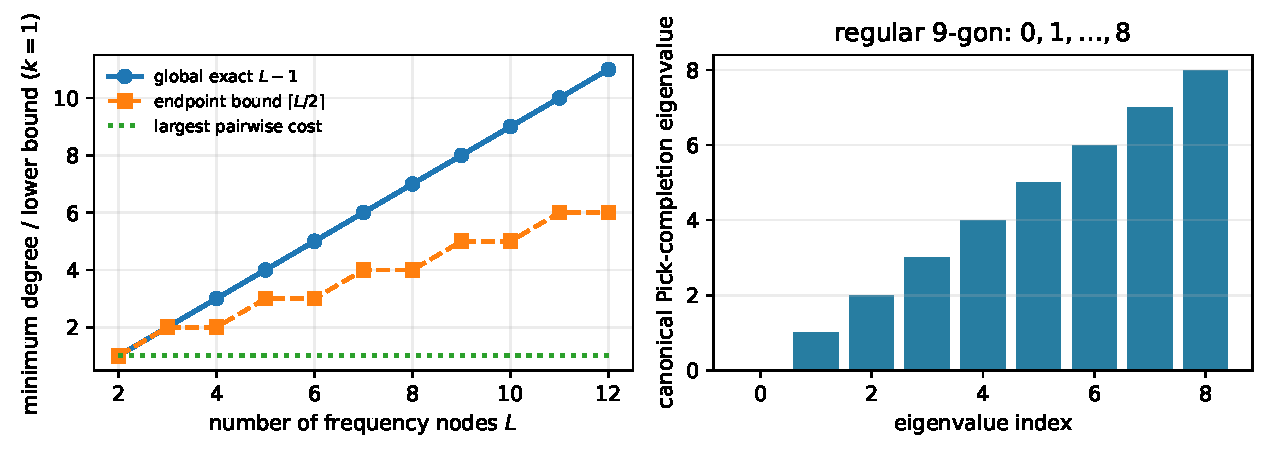
\includegraphics[width=0.94\linewidth]{figures/global_fanout_memory.pdf}
 \caption{Left: for one channel, the exact global degree $L-1$ grows above
 both the largest pairwise cost and the degree inferred by summing endpoint
 speed-limit bounds.  Right: at nine equally spaced nodes, the canonical Pick
 completion has the exact spectrum $0,1,\ldots,8$.}
 \label{fig:fanout}
\end{figure}

\section{Explicit regular-polygon completion}

Let $\omega=\e^{2\pi\mathrm i/L}$ and $\zeta_j=\omega^j$.  The matrix $C$ in
\eqref{eq:Cmatrix} is circulant.  A finite geometric-series calculation on
the Fourier vectors gives
\begin{equation}\label{eq:C-spectrum}
 \operatorname{spec}C=
 \left\{-\frac{L-1}{2},-\frac{L-3}{2},\ldots,
                    \frac{L-3}{2},\frac{L-1}{2}\right\}.
\end{equation}
Consequently
\begin{equation}\label{eq:pick-spectrum}
 P_0=\left(C+\frac{L-1}{2}I_L\right)\otimes I_k,
 \qquad
 \operatorname{spec}P_0=\{0,1,\ldots,L-1\}\text{ repeated $k$ times}.
\end{equation}
This is an exact certificate of rank $k(L-1)$.

Factor $P_0=F^*F$ and use the lurking pairs from
\cref{prop:pick-rank}.  Extending their isometry gives a unitary colligation
\[
                 \mathcal U=\begin{pmatrix}A&B\\C_0&D\end{pmatrix}
                 \quad\text{on }\C^{k(L-1)}\oplus\C^{Lk}
\]
and the transfer
\begin{equation}\label{eq:transfer}
                    S(z)=D+zC_0(I-zA)^{-1}B.
\end{equation}
Here the ambient output space has been chosen minimally as $N=Lk$; for
$N>Lk$, replace the second summand by $\C^N$.  After deleting decoupled
unit-circle state modes, each $I-\zeta_iA$ is invertible.  The lower bound
prevents any loss of state dimension,
so the controllable and observable part has exactly $k(L-1)$ states.

For arbitrary distinct nodes the same algorithm uses
$C-\lambda_{\min}(C)I$.  No optimization over diagonal blocks is required:
one eigenvalue computation, one Gram factorization and one unitary completion
produce a minimum-degree solution.

\section{Reproducible implementation audit}

The proofs are analytic; computation targets the interfaces most likely to
hide a sign, rank or regularity error.  The producer and verifier are separate
programs, and the verifier imports no producer functions.  The frozen
campaign contains:
\begin{itemize}
 \item the exact regular-polygon spectrum for $L=2,\ldots,24$;
 \item $384$ arbitrary-node completions with $3\le L\le12$, plus four
conditioning fixtures with node gaps down to $10^{-9}$;
 \item five explicit minimal colligations, including $(L,k)=(5,2)$ with
 eight controllable and observable states;
 \item $1{,}024$ noisy inertia trials, half exact fan-out alternatives and
 half null controls;
 \item $512$ independently perturbed near-orthogonal frame families, plus
strict-threshold fixtures up to $\norm{G-I}=0.999999$ and equality controls.
\end{itemize}

Across the arbitrary-node campaign there are zero rank failures.  The maximum
Stein residual is below $1.2\times10^{-14}$ and the maximum numerical PSD
violation below $6.1\times10^{-14}$.  The largest interpolation error among
the synthesized colligations is below $1.1\times10^{-14}$; all prescribed
state dimensions are both controllable and observable.  The noisy campaign
has zero false certificates and zero missed full certificates.  In the
near-orthogonal random campaign, the largest observed $\norm{G-I}$ is
$0.111<1$ and all $512$ cases retain the exact negative-inertia count.
Deterministic fixtures retain all $k(L-1)$ negative directions at
$\norm{G-I}=0.999999$; at equality, where two target planes coincide, exactly
$k$ compulsory directions disappear.  The noisy trials are implementation
checks of the fail-closed Weyl count, not statistical evidence.  These
numbers audit the implementation and do not replace the proofs.

\begin{table}[t]
\centering
\small
\begin{tabular}{@{}ccccc@{}}
\toprule
$(L,k)$ & pairwise degree & endpoint-bound count & exact degree
& max interpolation error \\
\midrule
$(3,1)$ & 1 & 2 & 2 & $3.2\times10^{-15}$ \\
$(4,1)$ & 1 & 2 & 3 & $7.7\times10^{-15}$ \\
$(5,1)$ & 1 & 3 & 4 & $9.0\times10^{-15}$ \\
$(4,2)$ & 2 & 4 & 6 & $1.1\times10^{-14}$ \\
$(5,2)$ & 2 & 5 & 8 & $9.4\times10^{-15}$ \\
\bottomrule
\end{tabular}
\caption{Minimal lurking-isometry realizations in the frozen artifact.}
\label{tab:colligations}
\end{table}

\section{Scope, falsifiers and physical reading}

The theorem concerns square finite rational-inner transfers, distinct
boundary nodes and a fixed input subspace.  Loss, gain, time variation,
singular inner factors and nonrational continuous-time propagation delays are
outside the class.  Repeated nodes require confluent interpolation.  McMillan
degree counts dynamical state dimension; converting it into fabrication
volume, thermodynamic work or monetary cost requires an additional physical
model.

The main result is falsifiable at three levels.  A positive completion of
rank below $k(L-1)$ would refute necessity.  Failure of the canonical
completion to produce a regular degree-$k(L-1)$ inner interpolant would refute
sufficiency.  A compatible noisy instance for which
\eqref{eq:noisy-count} overcounts the true degree would refute the robust
certificate.  The released tests audit the algebraic identities, the sharp
completion, independent colligation synthesis and the fail-closed count.

Operationally, the theorem says that a passive device cannot reuse one small
state space independently for arbitrarily many orthogonal frequency routes.
Each new orthogonal destination adds exactly $k$ states except the first.
The conclusion is architecture independent inside the rational-inner class:
it does not depend on a cascade, lattice, cavity or delay-line
implementation.  Near-orthogonal outputs require at least the same number of
states while their collective Gram perturbation remains below the explicit
threshold; exact attainability away from orthogonality is not claimed.

\section{Conclusion}

Pairwise spectral routing is not compositional.  At $L$ distinct frequencies,
routing one $k$-channel input to $L$ mutually orthogonal outputs costs exactly
$k(L-1)$ internal states, although every pair costs only $k$.  The law holds
at arbitrary node spacings, is attained by a closed Pick completion, and has
both an elementary minor-zero converse and a robust inertia converse.

The general identity
\[
              P-Z^*PZ=J_L\otimes I_k-G
\]
turns measured cross-frequency coherence into a direct lower bound on hidden
memory.  It also explains why summing endpoint-only Grassmann speed limits
cannot close the multi-node problem: geometry prices each arc, while Pick inertia prices the
compatibility of all arcs inside one analytic network.  The resulting
largest-pair/global gap grows without bound, and the endpoint-bound/global gap
approaches a factor of two.

Two next questions are now sharply posed: characterize exact attainability
for nonorthogonal Gram geometries, and combine the inertia coordinate with a
full multi-arc action region.  Neither is needed for the present fan-out law.

\section*{Data and code availability}

The manuscript, deterministic certificate, independent verifier, figure and
hash manifest are archived in the
\href{https://github.com/lluiseriksson/finite-sample-spectral-certificates/releases/tag/v2.1-global-fanout-memory-submission}{immutable GitHub release}.  The main entry points are
\path{research/global_fanout_memory_certificate.py} and
\path{verification/verify_global_fanout_memory.py}.  Seeds, tolerances and
all reported diagnostics are frozen in the JSON certificate.

\appendix

\section{Proof details for the finite-zero budget}

Write a rank-one Potapov factor as
\[
                  F_\ell(z)=I+(b_\ell(z)-1)p_\ell,
\]
where $p_\ell$ has rank one and $b_\ell$ is scalar Blaschke of degree one.
For fixed values of the other scalar coordinates, the full product is affine
in $b_\ell$ through a rank-one matrix.  If $M(t)=M_0+tuv^*$, every term in
the Leibniz expansion of $\det M(t)$ containing two entries from $uv^*$
vanishes, so $\det M(t)$ is affine in $t$.  Thus
$\det(U^*S(z)V)$ is multiaffine in the $n$ scalar Blaschke coordinates.
Putting the coordinates over their common denominator yields a scalar
numerator of degree at most $n$.

If an analytic $k$-by-$k$ matrix $H$ satisfies $H(z_0)=0$, write
$H(z)=(z-z_0)\widetilde H(z)$.  Its determinant contains the factor
$(z-z_0)^k$.  This proves the multiplicity statement used in the first
converse without a genericity or transversality assumption.

\section{The inertia lemma and its noisy form}

Let $A,B\succeq0$ on an $m$-dimensional space.  Any subspace on which
$A-B$ is negative definite intersects $\ker B$ trivially, because
$x^*(A-B)x=x^*Ax\ge0$ on $\ker B$.  Hence its dimension is at most
$\operatorname{codim}\ker B=\rank B$, proving
\[
                         \nminus(A-B)\le\rank B.
\]
For a Hermitian perturbation $\widehat H=H+E$ with $\norm E\le\eta$,
Weyl's inequality gives
$\lambda_j(H)\le\lambda_j(\widehat H)+\eta$.  Every observed eigenvalue
strictly below $-\eta$ therefore corresponds to a truly negative eigenvalue,
which proves \cref{cor:noisy}.

\section{Fourier diagonalization at equally spaced nodes}

For $\omega=\e^{2\pi\mathrm i/L}$, the first row of $C$ is
$0,(1-\omega)^{-1},\ldots,(1-\omega^{L-1})^{-1}$.  Testing the Fourier vector
$(1,\omega^{-m},\ldots,\omega^{-(L-1)m})$ and pairing the terms $j$ and
$L-j$ gives
\[
 \sum_{j=1}^{L-1}\frac{\omega^{-mj}}{1-\omega^j}
 =\frac{L-1}{2}-m,
 \qquad m=0,\ldots,L-1,
\]
with the opposite Fourier convention reversing the order.  This proves
\eqref{eq:C-spectrum} and \eqref{eq:pick-spectrum}.

\section{Verification contract}

\begin{table}[ht]
\centering
\small
\begin{tabular}{@{}lll@{}}
\toprule
Interface & Independent invariant & Frozen tolerance \\
\midrule
Regular polygon & spectrum $0,1,\ldots,L-1$ & $2\times10^{-11}$ \\
Arbitrary nodes & PSD, rank and Stein residual & $2\times10^{-10}$ \\
Colligation & unitarity, interpolation and minimality & $3\times10^{-7}$ \\
Noisy inertia & alternatives and null controls & zero count failures \\
Near orthogonality & $\norm{G-I}<1$ and inertia & zero count failures \\
Strict boundary & $0.999999$ and equality controls & exact inertia counts \\
\bottomrule
\end{tabular}
\caption{Fail-closed numerical contract.}
\label{tab:verification}
\end{table}

\bibliographystyle{plain}
\bibliography{references}

\end{document}
